\section{Rigid Bodies}

\begin{definition}[Rigid body]
    A \textbf{rigid body} is an extended object, consisting of $N$ particles that are constrained such that the distance between any pair of particles, $|\mathbf{r}_i - \mathbf{r}_j|$, is fixed. 
\end{definition}

The possible motions of a rigid body are the continuous isometries of Euclidean space, i.e. translations and rotations. Reflections change the ordering of intrisic structure of the rigid body so they are not included.

\subsection{Angular velocity}

Recall that if a particle is rotating about an axis through $O$ with angular velocity $ \boldsymbol{\omega} $ then the velocity $ \dot{\bfr} = \boldsymbol{\omega}\times \bfr $ with $ |\dot{\bfr}|=\omega r_\perp  $, where $ r_\perp  $ is the perpendicular distance to the axis of rotation.

If the particle has mass $m$, then the kinetic energy $T$ is 
\[
    T = \frac{1}{2}m|\dot{\mathbf{r}}|^2 = \frac{1}{2}m (\boldsymbol{\omega}\times \bfr)\cdot (\boldsymbol{\omega}\times \bfr) = \frac{1}{2}{\color{blue}mr_\perp^2} \omega^2 = \frac{1}{2}{\color{blue}I} \omega^2 .
\]
\begin{note}
    If $ \boldsymbol{\omega}=\omega \bfn $ then $ r_\perp = |\mathbf{n}\times \mathbf{r}| $.
\end{note}

\begin{definition}[Moment of inertia]
    The \textbf{moment of inertia} of a particle is
    \[
      I = m r_\perp^2 = m|\mathbf{n}\times \mathbf{r}|^2,
    \]
\end{definition}

\subsection{Moment of inertia}

Consider a rigid body made up of $N$ particles. Consider the body to be rotating about an axis through the origin with angular velocity $ \boldsymbol{\omega} $. Then for each particle 
\[
    \dot{\mathbf{r}}_i = \boldsymbol\omega\times \mathbf{r}_i.
\]
This ensures $ |\mathbf{r}_i-\mathbf{r}_j| $ does not vary with time:
\[
  \frac{\rmd }{\rmd t}|\mathbf{r}_i - \mathbf{r}_j|^2 = 2(\dot{\mathbf{r}}_i - \dot{\mathbf{r}}_j)\cdot (\mathbf{r}_i - \mathbf{r}_j) = 2\big(\boldsymbol\omega\times (\mathbf{r}_i - \mathbf{r}_j)\big) \cdot (\mathbf{r}_i - \mathbf{r}_j) = 0,
\]

Similarly, the kinetic energy is
\[
  T = \frac{1}{2}\sum_{i = 1}^N m_i|\dot{\mathbf{r}_i}|^2 =\frac{1}{2}\sum_{i = 1}^N m_i |\boldsymbol\omega\times \mathbf{r}_i|^2 = \frac{1}{2}\omega^2 {\color{blue}\sum_{i = 1}^N m_i  |\bfn \times \bfr_i|^2} = \frac{1}{2}{\color{blue}I}\omega^2.
\]
\begin{definition}[Moment of inertia]
    The \textbf{moment of inertia} of a rigid body about the rotation axis $\mathbf{n}$ is
    \[
      I = \sum_{i = 1}^N m_i(r_i)_{\perp}^2 = \sum_{i = 1}^N m_i  |\bfn \times \bfr_i|^2.
    \]
\end{definition}
\begin{definition}[Angular momentum]
    The \textbf{angular momentum} is
    \[
      \mathbf{L} = \sum_{i=1}^N m_i \mathbf{r}_i \times \dot{\mathbf{r}}_i = \sum_{i=1}^N m_i \mathbf{r}_i \times \boldsymbol\omega \times \mathbf{r}_i.
    \]
\end{definition}

Consider $ \boldsymbol{\omega}=\omega \mathbf{n} $, then 
\[
    \mathbf{L} = \omega \sum_{i=1}^N m_i (\mathbf{r}_i \times (\mathbf{n} \times \mathbf{r}_i)).
\]
Consider the part of $ \bfL $ parallel to the rotation of axis: 
\begin{align*}
    \mathbf{L} \cdot \mathbf{n} &= \omega \sum_{i=1}^N m_i \mathbf{n}\cdot (\mathbf{r}_i \times (\mathbf{n} \times \mathbf{r}_i))\\
    &= \omega \sum_{i=1}^N m_i(\mathbf{n}\times \mathbf{r}_i)\cdot (\mathbf{n} \times \mathbf{r}_i)\\
    &= \omega \sum_{i=1}^{N}m_i(r_i)_{\perp}^2 = I\omega.
\end{align*}
So component of angular momentum in direction of rotation axis is $ I \omega $. In general $ \mathbf{L} $ is \textit{not} $\parallel$ to rotation axis. But we can write 
\[
  \mathbf{L} = \sum_{i=1}^N m_i\big((\mathbf{r}_i\cdot \mathbf{r}_i)\boldsymbol \omega - (\mathbf{r}_i \cdot \boldsymbol\omega)\mathbf{r}_i\big),
\]
which is linear of $\boldsymbol\omega$. So we can write
\[
  \mathbf{L} = I \cdot \boldsymbol \omega,
\]
where we abuse notation to use $I$ for the \textbf{inertia tensor}. In suffix notation $ L_i = I_{ij}\omega_j $. Note that $I$ is a \textit{symmetric} tensor with components
\[
  I_{jk} = \sum_{i=1}^N m_i(|\mathbf{r}_i|^2 \delta_{jk} - (\mathbf{r}_i)_j(\mathbf{r}_i)_k),
\]
In general, there are 3 directions such that $ I \boldsymbol{\omega} \parallel \boldsymbol{\omega} $, which corresponds to \textbf{principal axes} of the tensor. If the body is rotated about a principal axis, then $\mathbf{L}\parallel \boldsymbol\omega$. Note that it holds for \textit{any} body.

Recap the simple case: if we choose to rotate in a direction such that $ \mathbf{L}\parallel \boldsymbol\omega $, then 
\[
    \bfL = I(\bfn) \boldsymbol{\omega},
\]
where $ I(\bfn) $ is the moment of inertia about $\bfn$. We often consider bodies that are \textit{symmetric} about a particular axis, and rotating about that axis guarantees above property. 

\subsection{Calculation of the moment of inertia}
For a solid body, we replace mass-weighted sums over particles by mass-weighted integrals. In particular, consider a body occupying a volumn $V$ with the mass density $\rho(\mathbf{r})$. Then 
\begin{definition}
    The \textbf{mass} is
    \[
      M = \int_V \rho(\mathbf{r}) \,\rmd V.
    \]
    The \textbf{centre of mass} is
    \[
      \mathbf{R} = \frac{1}{M}\int_V \mathbf{r}\rho(\mathbf{r})\,\rmd V.
    \]
    The \textbf{moment of inertia} about axis $\bfn$ is
    \[
      I = \int_V \rho(\mathbf{r}) r_{\perp}^2 \,\rmd V = \int_V \rho(\mathbf{r})|\mathbf{n}\times \mathbf{r}|^2\,\rmd V.
    \]
\end{definition}
Use the obvious modifications of these formulae for bodies that corresponds to mass distributed over a surface or along a curve, as surface(area) integrals or line integrals.

\begin{example}
    Consider a uniform ring of mass $M$ and radius $a$, about an axis through the centre, perpendicular to the plane of the ring.
    \begin{center}
      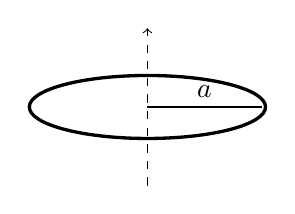
\begin{tikzpicture}
        \draw [dashed,->] (0, -1) -- (0, 1);
        \draw [very thick] circle [x radius = 1.5, y radius = 0.4];
        \draw (0, 0) -- (1.45, 0) node [pos = 0.5, above] {$a$};
      \end{tikzpicture}
    \end{center}
    In this case we reduce to a line integral and $ \rho = M/2\pi a $. $ r_{\perp }=a $, so 
    \[
      I = \int_{0}^{2\pi} \underbrace{\frac{M}{2\pi a}}_{\rho} \underbrace{a^2}_{r_{\perp}^2} \underbrace{a \dd \theta}_{\rmd s}= Ma^2.
    \]
\end{example}

\begin{example}
    Consider a uniform rod of mass $M$ and length $l$ with axis through one end, perpendicular to the rod.
    \begin{center}
      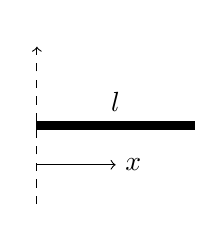
\begin{tikzpicture}
        \draw [dashed,->] (0, -1) -- (0, 1) node [above] {$\bfn$};
        \filldraw[black] (0, 0.05) rectangle (2, -0.05);
        \node at (1, 0.3) {$l$};
        \draw [->] (0,-0.5) -- (1,-0.5) node [right] {$x$};
      \end{tikzpicture}
    \end{center}
    $\rho = M/l$. So the moment of inertia is
    \[
      I = \int_0 ^l \frac{M}{l}x^2\dd x = \frac{1}{3}Ml^2.
    \]
\end{example}

\begin{example}
  Consider a disc of mass $M$ and radius $a$, with a rotation axis through the centre, perpendicular to the plane of the disc.
  \begin{center}
    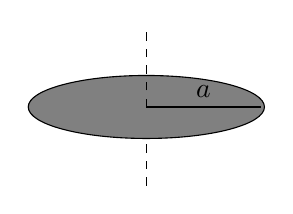
\begin{tikzpicture}
      \draw [fill=gray] circle[x radius = 1.5, y radius = 0.4];
      \draw (0, 0) -- (1.45, 0) node [pos = 0.5, above] {$a$};
      \draw [dashed] (0, -1) -- (0, -0.4);
      \draw [dashed] (0, 0) -- (0, 1);
    \end{tikzpicture}
  \end{center}
  Then
  \begin{align*}
    I &= \int_{0}^{2\pi}\int_0^a \underbrace{\frac{M}{\pi a^2}}_{\rho} \underbrace{r^2}_{r_\perp^2} \underbrace{r\dd r\dd \theta}_{\dd A}\\
    &= \frac{M}{\pi a^2}\int_0^a r^3\dd r \int_0^{2\pi}\dd \theta\\
    &= \frac{M}{\pi a^2}\frac{1}{4}a^4 (2\pi)\\
    &= \frac{1}{2}Ma^2.
  \end{align*}
  Now suppose that the rotation axis is in the plane of the disc instead (also rotating through the centre). Then
  \begin{align*}
    I &= \int_{0}^{2\pi}\int_0^a \underbrace{\frac{M}{\pi a^2}}_{\rho} \underbrace{(r\sin \theta)^2}_{r_\perp^2} \underbrace{r\dd r\dd \theta}_{\dd A}\\
    &= \frac{M}{\pi a^2}\int_0^a r^3\dd r \int_0^{2\pi}\sin^2 \theta\dd \theta\\
    &= \frac{M}{\pi a^2}\frac{1}{4}a^4 \pi\\
    &= \frac{1}{4}Ma^2.
  \end{align*}
\end{example}

\begin{example}
  Consider a solid sphere with mass $M$, radius $a$, with a rotation axis though the centre.
  \begin{center}
    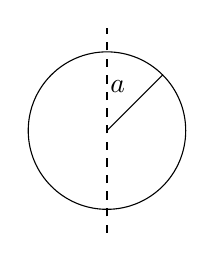
\begin{tikzpicture}
      \draw circle [radius = 1];
      \draw (0, 0) -- (0.707, 0.707) node [pos =0.5, anchor = south east] {$a$};
      \draw [dashed] (0, -1.3) -- (0, 1.3);
    \end{tikzpicture}
  \end{center}
  Using spherical polar coordinates $(r, \theta, \phi)$ based on the rotation axis,
  \begin{align*}
    I &= \int_{0}^{2\pi}\int_0^\pi\int_0^a \underbrace{\frac{M}{\frac{4}{3}\pi a^3}}_{\rho}\underbrace{(r\sin \theta)^2}_{r_\perp^2} \underbrace{r^2\sin \theta\dd r\dd \theta\dd \phi}_{\dd V}\\
    &= \frac{M}{\frac{4}{3}\pi a^3}\int_0^a r^4 \dd r\int_0^\pi (1 - \cos^2)\sin \theta\dd \theta \int_0^{2\pi}\dd \phi\\
    &= \frac{M}{\frac{4}{3}\pi a^3}\cdot \frac{1}{5}a^5 \cdot \frac{4}{3}\cdot 2\pi\\
    &= \frac{2}{5}Ma^2.
  \end{align*}
\end{example}

Usually, finding the moment of inertia involves doing complicated integrals. We will now come up with two theorems that help us find moments of inertia.
\begin{theorem}[Perpendicular axis theorem]
  For a two-dimensional object (a lamina), and three perpendicular axes $x, y, z$ through the same spot, with $z$ normal to the plane,
  \[
    I_z = I_x + I_y,
  \]
  where $I_z$ is the moment of inertia about the $z$ axis.
  \begin{center}
    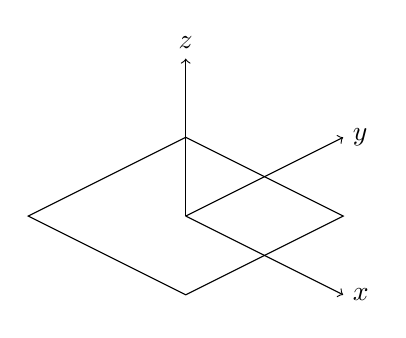
\begin{tikzpicture}
      \draw [->] (0, 0) -- (2, -1) node [right] {$x$};
      \draw [->] (0, 0) -- (2, 1) node [right] {$y$};
      \draw [->] (0, 0) -- (0, 2) node [above] {$z$};
      \draw (-2, 0) -- (0, -1) -- (2, 0) -- (0, 1) -- cycle;
    \end{tikzpicture}
  \end{center}
\end{theorem}
Note that this does \emph{not} apply to 3D objects! For example, in a sphere, $I_x = I_y = I_z$.

\begin{proof}
  Let $\rho$ be the mass per unit volume. Then
  \begin{align*}
    I_x &= \int_A \rho y^2 \dd A\\
    I_y &= \int_A \rho x^2 \dd A\\
    I_z &= \int_A \rho (x^2 + y^2)\dd A = I_x + I_y.\qedhere
  \end{align*}
\end{proof}
\begin{example}
  For a disc, $I_x = I_y$ by symmetry. So $I_z = 2 I_x$.
\end{example}

\begin{theorem}[Parallel axis theorem]
  If a rigid body of mass $M$ has moment of inertia $I_C$ about an axis passing through the centre of mass, then its moment of inertia about a parallel axis a distance $d$ away is
  \[
    I = I_C + Md^2.
  \]
  \begin{center}
    \begin{tikzpicture}
      \draw plot [smooth cycle] coordinates{(0, 0) (1, -2) (3, -1) (4, 0) (4, 1) (2, 1) (1, 3)};
      \node [dot=3pt] at (2, 0) {};
      \node at (2, 0) [left] {CoM};
      \draw [dashed] (2, -2.5) -- (2, 3);
      \draw [dashed] (3, -2.5) -- (3, 3);
      \draw [->] (2, 0) -- (3, 0);
      \draw [->] (3, 0) -- (2, 0) node [pos = 0.5, above] {$d$};
    \end{tikzpicture}
  \end{center}
\end{theorem}

\begin{proof}
  With a convenient choice of Cartesian coordinates such that the centre of mass is at the origin and the two rotation axes are $x = y =0$ and $x = d, y = 0$,
  \[
    I_C = \int_V \rho (x^2 + y^2) \dd V,
  \]
  so
  \begin{align*}
    I &= \int_V \rho((x - d)^2 + y^2)\dd V\\
    &=\int_V \rho (x^2 + y^2)\dd V - 2d\int_V \rho x\dd V + \int_V d^2 \rho\dd V\\
    &= I_C + 0 + Md^2\\
    &= I_C + Md^2.\qedhere
  \end{align*}
\end{proof}
\begin{example}
  Take a disc of mass $M$ and radius $a$, and rotation axis through a point on the circumference, perpendicular to the plane of the disc. Then
  \begin{center}
    \begin{tikzpicture}
      \draw [fill=gray] circle [x radius = 2, y radius = 0.6];
      \node [dot] {};
      \draw (0, 0) -- (1.03, 0.5) node [pos = 0.5, anchor = south east] {$a$};
      \draw [dashed] (2, -1) -- (2, 1);
    \end{tikzpicture}
  \end{center}
  \[
    I = I^c + Ma^2 = \frac{1}{2}Ma^2 + Ma^2 = \frac{3}{2}Ma^2.
  \]
\end{example}

\subsection{Motion of a rigid body}
The general motion of a rigid body can be described as a translation of its centre of mass, following a trajectory $\mathbf{R}(t)$, together with a rotation about an axis through the centre of mass. As before, we write
\[
  \mathbf{r}_i = \mathbf{R} + \mathbf{s}_i,\quad\dot{\mathbf{r}}_i = \dot{\mathbf{R}} + \dot{\mathbf{s}}_i. 
\]
If the body rotates with angular velocity $\boldsymbol\omega$ about the centre of mass, then
\[
  \dot{\mathbf{s}}_i = \boldsymbol\omega \times \mathbf{s}_i.
\]
Since $\mathbf{s}_i = \mathbf{r}_i - \mathbf{R}$, we have
\[
  \dot{\mathbf{r}_i} = \dot{\mathbf{R}} + \boldsymbol \omega \times \mathbf{s}_i = \dot{\mathbf{R}} + \boldsymbol\omega\times (\mathbf{r}_i - \mathbf{R}).
\]
On the other hand, the kinetic energy, as calculated in previous lectures, is
\begin{align*}
  T &= \frac{1}{2}M|\dot{\mathbf{R}}|^2 + \frac{1}{2}\sum_i m_i |\dot{\mathbf{s}}_i|^2\\
  &= \underbrace{\frac{1}{2}M|\dot{\mathbf{R}}|^2}_{\text{translational $T$}} + \underbrace{\frac{1}{2}I_C\omega^2}_{\text{rotational $T$}}.
\end{align*}

Sometimes we do not want to use the centre of mass as the centre. For example, if an item is held at the edge and spun around, we'd like to study the motion about the point at which the item is held, and not the centre of mass.

So consider any point $Q$, with position vector $\mathbf{Q}(t)$ that is not the centre of mass but moves with the rigid body, i.e.
\[
  \dot{\mathbf{Q}} = \dot{\mathbf{R}} + \boldsymbol\omega\times (\mathbf{Q} - \mathbf{R}).
\]
Usually this is a point inside the object itself, but we do not assume that in our calculation.

Then we can write
\begin{align*}
  \dot{\mathbf{r}}_i &= \dot{\mathbf{R}} + \boldsymbol\omega\times (\mathbf{r}_i - \mathbf{R})\\
  &= \dot{\mathbf{Q}} - \boldsymbol\omega\times (\mathbf{Q} - \mathbf{R}) + \boldsymbol\omega \times (\mathbf{r}_i - \mathbf{R})\\
  &= \dot{\mathbf{Q}} + \boldsymbol\omega\times (\mathbf{r}_i - \mathbf{Q}).
\end{align*}
Therefore the motion can be considered as a translation of $Q$ (with \emph{different} velocity than the centre of mass), together with rotation about $Q$ (with the \emph{same} angular velocity $\boldsymbol\omega$).

\subsubsection*{Equations of motion}
As shown previously, the linear and angular momenta evolve according to
\begin{align*}
  \dot{\mathbf{P}} &= \mathbf{F}\quad \text{(total external force)}\\
  \dot{\mathbf{L}} &= \mathbf{G}\quad \text{(total external torque)}
\end{align*}
These two equations determine the translational and rotational motion of a rigid body.

$\mathbf{L}$ and $\mathbf{G}$ depend on the choice of origin, which could be any point that is fixed in an inertial frame. More surprisingly, it can also be applied to the centre of mass, even if this is accelerated.

Indeed, 
\begin{align*}
  \bfG&=\frac{\mathrm{d}}{\mathrm{d}t}\left( M\bfR\times\dot{\bfR}+\sum_{i=1}^{N}m_i\bfs_i\times \dot{\bfs}_i \right)\\ 
  &= M\bfR \times \ddot{\bfR} + \frac{\mathrm{d}}{\mathrm{d}t}\left( \sum_{i=1}^{N}m_i\bfs_i\times \dot{\bfs}_i \right)\\ 
  &= \bfR \times \bfF^{\text{ext}} +\frac{\mathrm{d}}{\mathrm{d}t}\left( \sum_{i=1}^{N}m_i\bfs_i\times \dot{\bfs}_i \right). 
\end{align*}
Hence 
\begin{align*}
  \frac{\mathrm{d}}{\mathrm{d}t}\left( \sum_{i=1}^{N}m_i\bfs_i\times \dot{\bfs}_i \right)&= \bfG-\bfR \times \bfF^{\text{ext}}\\ 
  &= \sum_{i=1}^{N}\bfr_i \times \bfF_i^{\text{ext}} - \bfR \times \bfF^{\text{ext}}\\ 
  &= \sum_{i=1}^{N}(\bfr_i-\bfR)\times \bfF_i^{\text{ext}},
\end{align*}
which is the total external torque, as claimed.

\subsubsection*{Motion in a uniform gravitational field}

In a uniform gravitational field $\mathbf{g}$, the total gravitational force and torque are the same as those that would act on a single particle of mass $M$ located at the centre of mass (which is also the \textbf{centre of gravity}):
\[
  \mathbf{F} = \sum_i \mathbf{F}_i^{\mathrm{ext}} = \sum_i m_i \mathbf{g} = M\mathbf{g},
\]
and 
\[
  \mathbf{G} = \sum_i \mathbf{G}_i^{\mathrm{ext}} = \sum_i \mathbf{r}_i \times (m_i \mathbf{g}) = \sum m_i \mathbf{r}_i \times \mathbf{g} = M\mathbf{R}\times \mathbf{g}.
\]
In particular, the gravitational torque about the center of mass vanishes: $\mathbf{G}_C = \mathbf{0}$.

We obtain a similar result for gravitational potential energy. The gravitational potential in a uniform $\mathbf{g}$ is
\[
  \Phi_g = -\mathbf{r}\cdot \mathbf{g}.
\]
(since $\mathbf{g} = -\nabla \Phi_g$ by definition). So
\[
  V^{\mathrm{ext}} = \sum_i V_i^{\mathrm{ext}}
  = \sum_i m_i (- \mathbf{r}_i \cdot \mathbf{g})
  = -M\bfR\cdot\bfg .
\]

\begin{example}
  Consider a stick thrown into the air. Then the center of the stick moves in a parabola. Meanwhile, the stick rotates with constant angular velocity about its center dueto the absence of torque.
\end{example}